\documentclass[9pt,xcolor=table,hyperref=unicode]{beamer}
\setbeamertemplate{background canvas}[vertical shading][bottom=red!10,top=blue!10]
\usetheme{Berkeley}
\usepackage[utf8]{vietnam}
\usepackage{tikz}
\usepackage{hyperref}
\usepackage{booktabs, multicol, multirow}
\usepackage{adjustbox}
\usepackage{array}
\newcolumntype{x}[1]{>{\centering\arraybackslash\hspace{0pt}}p{#1}}
\graphicspath{ {images/} }
\usepackage{xcolor}

\setbeamerfont{page number in head/foot}{size=\tiny}
\setbeamertemplate{footline}[frame number]

\newcommand{\inlineitem}{%
\leavevmode\usebeamertemplate{itemize item}
}
\newcounter{newenumi}
\setcounter{newenumi}{1}

\newcommand{\inlineenum}{%
 {%
 \setcounter{enumi}{\thenewenumi}%
 \leavevmode\usebeamertemplate{enumerate  item}
 \stepcounter{newenumi}
 \setcounter{enumi}{0}
 }
}

\newcommand{\resetinlineenum}{
 \setcounter{newenumi}{1}
}

\begin{document}
	\setbeamertemplate{sidebar left}[sidebar theme]
	
	\title{Luận văn tốt nghiệp}
	\subtitle{Phân giải đồng tham chiếu cho các đối tượng và thuộc tính trong khai khoáng ý kiến}
	\author[]{
		\begin{tabular}{ll}
			Nguyễn Trọng Nghĩa & 51202370 \\
			Nguyễn Đăng Trang & 51203957 \\
			 & 
		\end{tabular}
		\break
		\begin{tabular}{ll}
			GVHD & GS.TS Phan Thị Tươi \\
			GVPB & GS.TS Cao Hoàng Trụ
		\end{tabular}
	}
	\institute{Đại học Bách Khoa TP. Hồ Chí Minh}
	\date{\today}
	
	\begin{frame}
		\Large
		\maketitle
	\end{frame}

	\begin{frame}{Nội dung trình bày}
		\LARGE
		\begin{itemize}			
			\item{Tổng quan đề tài}
			\item{Các công trình liên quan}
			\item{Phương pháp đề xuất}
			\item{Thực nghiệm và đánh giá}
			\item{Tổng kết}
		\end{itemize}
	\end{frame}


	\section{Tổng quan đề tài}
	\begin{frame}
		\frametitle{Tổng quan đề tài}
		\begin{block}{Giới thiệu đề tài}
			\begin{itemize}
				\item{\textbf{Phân giải đồng tham chiếu} là một chủ đề trong lĩnh vực Xử lý ngôn ngữ tự nhiên. Mục tiêu là tìm kiếm những từ, cụm từ hoặc ngữ cùng chỉ đến một khái niệm, thực thể trong thế giới thực.}
				\item{\textbf{Phân giải đồng tham chiếu cho đối tượng và thuộc tính trong khai khoáng ý kiến} hướng đến việc phân giải đồng tham chiếu cho các đối tượng và thuộc tính trong văn bản chứa ý kiến.}
			\end{itemize}
		\end{block}		

		\begin{block}{Ví dụ}
		\begin{itemize}
			\item{\textit{Beckham} will visit Vietnam tomorrow. \textit{He} will attend a football event in Saigon.}
			\item{\textit{The Samsung Galaxy S3} is one of the best phones I’ve ever used. I absolutely
love the phone and \textit{the photo quality} \underline{it} has.}
		\end{itemize}
		\end{block}		
	\end{frame}


	\section{Tổng quan đề tài}
	\begin{frame}
		\begin{block}{Động cơ thực hiện đề tài}
			\begin{itemize}	
				\item{Thương mại điện tử đang phát triển mạnh mẽ và người dùng có nhu cầu thể hiện ý kiến lên các sản phẩm trên mạng. Ý kiến thường hướng đến đối tượng và thuộc tính; trong đó đối tượng là sản phẩm, thuộc tính là bộ phận hoặc đặc tính của sản phẩm.}
				\item{Nếu không có phân giải đồng tham chiếu cho các đối tượng và thuộc tính, ý kiến của người viết rất có thể sẽ được gán không đúng cho các thực thể.}
				\item{Cải thiển 10\% kết quả Khai khoáng ý kiến (theo Nicolas Nicolov).}
			\end{itemize}		
		\end{block}		
	\end{frame}

% 	\section{Tổng quan đề tài}
% 	\begin{frame}
% 		\frametitle{Tổng quan đề tài}
% 		\begin{block}{Động cơ}
% 			\textbf{Phân giải đồng tham chiếu cho đối tượng và thuộc tính trong khai khoáng ý kiến} hướng đến việc phân giải đồng tham chiếu cho các đối tượng và thuộc tính trong văn bản chứa ý kiến.	
% 			\begin{itemize}	
% 				\item{Thương mại điện tử đang phát triển mạnh mẽ và người dùng có nhu cầu thể hiện ý kiến lên các sản phẩm trên mạng.}			
% 				\item{Đối tượng và thuộc tính là các thực thể được thể hiện ý kiến, trong đó thuộc tính là bộ phận hoặc đặc tính của đối tượng.}
% 				\item{Nếu không có phân giải đồng tham chiếu cho các đối tượng và thuộc tính, ý kiến của người viết rất có thể sẽ được gán không đúng cho các thực thể.}
% 			\end{itemize}		
% 		\end{block}		
% 	\end{frame}

% 	\begin{frame}{Tổng quan đề tài (tt)}
% 		\begin{block}{Phân giải đồng tham chiếu}			
% 			\textbf{Phân giải đồng tham chiếu} là một bài toán kinh điển trong Xử lý ngôn ngữ tự nhiên. Mục tiêu của bài toán là tìm kiếm những từ, cụm từ hoặc ngữ cùng chỉ đến một khái niệm, thực thể trong thế giới thực. 
% 		\end{block}
% 		\begin{block}{Ví dụ}
% 		\begin{itemize}
% 			\item{\textit{Beckham} will visit Vietnam tomorrow. \textit{He} will attend a football event in Saigon.}
% 			\item{\textit{The Samsung Galaxy S3} is one of the best phones I’ve ever used. I absolutely
% love the phone and \textit{the photo quality} \underline{it} has.}
% 		\end{itemize}
% 		\end{block}		
% 	\end{frame}


	\begin{frame}
		\frametitle{Tổng quan đề tài (tt)}
		\begin{block}{Mục tiêu đề tài}
			Tìm ra các từ/cụm từ trong văn bản chứa ý kiến cùng chỉ về một đối tượng hoặc thuộc tính nào đó, tức là tìm các chuỗi đồng tham chiếu của đối tượng và thuộc tính.
		\end{block}		
		\begin{block}{Phạm vi đề tài}
			\begin{itemize}
				\item{Giả định rằng các đối tượng và thuộc tính đã được tìm ra}
				\item{Chỉ xét các quan hệ đồng tham chiếu dạng \textit{đồng nhất (identity)}}
			\end{itemize}
		\end{block}
	\end{frame}


	\section{Các công trình liên quan}
	\begin{frame}
		\frametitle{Các công trình liên quan}
		\begin{block}{Đồng tham chiếu}
			Kể từ những năm 1960 đến nay đã nhiều công trình nghiên cứu, với nhiều mô hình, nhiều hướng tiếp cận giải quyết khác nhau.
		\end{block}
		\begin{block}{Đồng tham chiếu trong khai khoáng ý kiến}
			\begin{itemize}
				\item{Stoyanov và Cardie (2006): Phân giải đồng tham chiếu cá nhân, tổ chức}
				\item{Hu và Liu (2010): Phân giải đồng tham chiếu đối tượng và thuộc tính}
			\end{itemize}
		\end{block}		
	\end{frame}

	\section{Phương pháp đề xuất}
	\subsection{Tổng quan quy trình}
	\begin{frame}{Tổng quan quy trình}		
		\begin{figure}[H]
			\LARGE 
			\centering				
			\resizebox{100mm}{!}{% Author: Rasmus Pank Roulund
% \documentclass{minimal}
% \usepackage{tikz}
% \usepackage[utf8]{vietnam}

% \begin{document}
% \usetikzlibrary{arrows,chains,positioning,scopes}

\tikzset{
    block/.style={draw,thick,text width=10em,minimum height=6.5em,minimum width=11em,align=center},
    arrow/.style={->, thick}
}
\begin{tikzpicture}
  {[start chain]
      \node[block,on chain] (N1) {Tập hợp các cụm danh từ};
      \node[block,on chain,join=by {arrow},right=1cm of N1] (N2) {Tiền xử lý};
      \node[block,on chain,join=by {arrow},right=1cm of N2] (N3) {Trích xuất cụm danh từ};
      \node[block,on chain,join=by {arrow},below=1cm of N3] (N4) {Xây dựng dữ liệu học và kiểm tra};
      \node[block,on chain,join=by {arrow},left=1cm of N4] (N5) {Xây dựng bộ phân loại và gom cụm};
      \node[block,on chain,join=by {arrow},left=1cm of N5] (N6) {Các chuỗi đồng tham chiếu};      
    }
      
  \end{tikzpicture}
% \end{document}}
			\caption{Tổng quan quy trình phân giải đồng tham chiếu}	
			\label{fig:generalmodel}						
		\end{figure}
	\end{frame}	

	\subsection{Tiền xử lý}	
	\begin{frame}{Tiền xử lý}		
		\begin{columns}[t]
			\begin{column}{0.4\textwidth}				
			   	\begin{block}{Tiền xử lý văn bản thô}
	   				Sửa lỗi chính tả và một số lỗi nhỏ khác do cách viết không chuẩn mực của người dùng.
				\end{block}
			\end{column}
			\begin{column}{0.6\textwidth}  %%<--- here				
			 	\begin{figure}[H]
					\LARGE 
					\centering				
					\resizebox{65mm}{!}{\input{images/GD_1.pdf_tex}}	
				\end{figure}				
			\end{column}
		\end{columns}
		\begin{columns}[t]
			\begin{column}{\textwidth}				
			   	\begin{block}{Tách câu, tách từ và gán nhãn từ loại}			   		
			   			\inlineitem{Dùng công cụ Stanford \footnotemark}
			   			\inlineitem{Dựa theo Penn Treebank POS Tag \footnotemark}		   			
				\end{block}
			\end{column}			
		\end{columns}
		\footnotetext[1]{http://stanfordnlp.github.io/CoreNLP}
		\footnotetext[2]{http://web.mit.edu/6.863/www/PennTreebankTags.html}
	\end{frame}

	\subsection{Trích xuất cụm danh từ}
	\begin{frame}{Trích xuất cụm danh từ}		
		\begin{columns}[t]
			\begin{column}{0.4\textwidth}
			   	\begin{block}{Tìm các cụm danh từ}
	   				Dựa vào công cụ CRFChunker \footnotemark.
				\end{block}
				\begin{block}{Lọc lại các cụm danh từ}
			   		Loại một số cụm danh từ vì chúng không thể chỉ về đối tượng hoặc thuộc tính.				
				\end{block}
			\end{column}
			\begin{column}{0.6\textwidth}  %%<--- here
			 	\begin{figure}[H]
					\LARGE 
					\centering				
					\resizebox{65mm}{!}{\input{images/GD_2.pdf_tex}}	
				\end{figure}
			\end{column}
		\end{columns}
		\footnotetext[3]{http://crfchunker.sourceforge.net}
		\begin{columns}[t]
			\begin{column}{\textwidth}
			   	\begin{block}{Gán nhãn cụm danh từ}					
					\textit{Ví dụ:} <0,-1,0 The Note 3> is a lot lighter than <1,-1,0 my HTC EVO>. <2,0,2 It>'s very fast and has <3,0,1 so many features> that <4,-1,0 an IPhone5> can't touch. 
				\end{block}					
			\end{column}			
		\end{columns}
	\end{frame}

	\subsection{Xây dựng dữ liệu học và kiểm tra}
	\begin{frame}{Xây dựng dữ liệu học và kiểm tra}				
		\begin{columns}[t]
			\begin{column}{0.4\textwidth}
			   	\begin{block}{Tạo các cặp cụm danh từ}
					Có ít nhất một đối tượng hoặc thuộc tính trong mỗi cặp cụm danh từ được tạo.
				\end{block}
			\end{column}
			\begin{column}{0.6\textwidth}  %%<--- here
			 	\begin{figure}[H]
					\LARGE 
					\centering				
					\resizebox{65mm}{!}{\input{images/GD_3.pdf_tex}}	
				\end{figure}
			\end{column}
		\end{columns}
		\begin{columns}[t]
			\begin{column}{\textwidth}
			   	\begin{block}{Tạo các vectơ đặc trưng}										
					$(<f_{1},f_{2},f_{3},…,f_{n}>, y)$
					\begin{itemize}
						\item{<$<f_{1},f_{2},f_{3},…,f_{n}>$: tập đặc trưng}
						\item{$y$: giá trị phân loại}										
					\end{itemize}
				\end{block}					
			\end{column}			
		\end{columns}
	\end{frame}	

	\begin{frame}{Xây dựng dữ liệu học và kiểm tra (tt)}		
		\begin{table}[]		
		\parbox{\textwidth}{
			\centering			
			\fontsize{6pt}{7}\selectfont		
			\begin{tabular}{|l|l|l|}
\hline
Nhóm thuộc tính                                                                               & Thuộc tính                                                                           & Giải thích                                                                                                                                                                                                                                   \\ \hline
\multirow{2}{*}{\begin{tabular}[c]{@{}l@{}}Nhóm liên quan \\ khai khoáng ý kiến\end{tabular}} & Tính nhất quán về ý kiến                                                             & \begin{tabular}[c]{@{}l@{}}Bằng 1 nếu NP1 và NP2 có\\ cùng thiên hướng ý kiến. \\ Bằng 0 nếu chúng khác về \\ thiên hướng ý kiến. \\ Nếu không xác định được \\ thiên hướngý kiến cho NP1 \\ hoặc NP2 thì bằng 2.\end{tabular} \\ \cline{2-3} 
                                                                                              & \begin{tabular}[c]{@{}l@{}}Sự kết hợp giữa thực thể \\ và từ chỉ ý kiến\end{tabular} & \begin{tabular}[c]{@{}l@{}}Bằng 0,1,2,3,4,10 tùy vào \\ xếp hạng PMI\end{tabular}                                                                                                                                                            \\ \hline
\multirow{6}{*}{\begin{tabular}[c]{@{}l@{}}Nhóm liên quan \\ ngữ pháp\end{tabular}}           & NP1 là đại từ                                                                    & \begin{tabular}[c]{@{}l@{}}Bằng 1 nếu NP1 là đại từ, \\ ngược lại bằng 0\end{tabular}                                                                                                                                                    \\ \cline{2-3} 
                                                                                              & NP2 là đại từ                                                                     & \begin{tabular}[c]{@{}l@{}}Bằng 1 nếu NP2 là đại từ, \\ ngược lại bằng 0\end{tabular}                                                                                                                                                     \\ \cline{2-3} 
                                                                                              & Tính thống nhất về số                                                                & \begin{tabular}[c]{@{}l@{}}Bằng 1 nếu NP1 và NP2 \\ thống nhất về số (trong ngữ pháp),\\  ngược lại bằng 0\end{tabular}                                                                                                               \\ \cline{2-3} 
                                                                                              & Từ hạn định                                                                          & \begin{tabular}[c]{@{}l@{}}Bằng 1 nếu NP2 bắt đầu bằng \\ "the", ngược lại bằng 0\end{tabular}                                                                                                                                            \\ \cline{2-3} 
                                                                                              & Từ chỉ trỏ                                                                           & \begin{tabular}[c]{@{}l@{}}Bằng 1 nếu NP2 bắt đầu bằng \\ "this", "that", "these", those", \\ ngược lại bằng 0\end{tabular}                                                                                                               \\ \cline{2-3} 
                                                                                              & \begin{tabular}[c]{@{}l@{}}Cả NP1 và NP2 \\ đều là tên riêng\end{tabular} & \begin{tabular}[c]{@{}l@{}}Bằng 1 nếu NP1 và NP2 \\ đều là tên riêng, ngược lại \\ bằng 0\end{tabular}                                                                                                                            \\ \hline
\begin{tabular}[c]{@{}l@{}}Nhóm liên quan \\ từ vựng\end{tabular}                             & Tương tự về từ vựng                                                                  & \begin{tabular}[c]{@{}l@{}}Tính tương tự về mặt từ vựng \\ (trùng hoặc gần giống nhau)\end{tabular}                                                                                                                                          \\ \hline
\multirow{3}{*}{Khác}                                                                         & Khoảng cách                                                                          & \begin{tabular}[c]{@{}l@{}}Khoảng cách về câu chứa NP1 \\ và NP2. Nếu chúng nằm cùng \\ một câu thì bằng 0\end{tabular}                                                                                                               \\ \cline{2-3} 
                                                                                              & Từ khóa "is" nằm ở giữa                                                              & \begin{tabular}[c]{@{}l@{}}Bằng 1 nếu có "is" không đi kèm \\ với chỉ định so sánh nào nằm ở \\ giữa NP1 và NP2, ngược lại \\ thì bằng 0\end{tabular}                                                                                 \\ \cline{2-3} 
                                                                                              & Từ khóa "has" nằm ở giữa                                                             & \begin{tabular}[c]{@{}l@{}}Bằng 1 nếu có "has" nằm ở giữa \\ NP1 và NP2, ngược lại thì \\ bằng 0\end{tabular}                                                                                                                         \\ \hline
\end{tabular}	
			\caption{Các đặc trưng được sử dụng trong hệ thống}
		}
		\end{table}
	\end{frame}	

	\begin{frame}{Xây dựng dữ liệu học và kiểm tra (tt)}		
		\begin{table}[]		
		\parbox{\textwidth}{
			\centering
			\fontsize{6pt}{7}\selectfont			
			\begin{tabular}{|l|l|l|}
\hline
Nhóm đặc trưng                                                                                & Đặc trưng                                                                            & Giải thích                                                                                                                                                                                                                      \\ \hline
\multirow{3}{*}{\begin{tabular}[c]{@{}l@{}}Nhóm liên quan\\ từ vựng\end{tabular}}             & Giống nhau hoàn toàn                                                                 & \begin{tabular}[c]{@{}l@{}}Bằng 1 nếu NP1 và NP2\\ giống nhau hoàn toàn về mặt\\ từ vựng\end{tabular}                                                                                                                           \\ \cline{2-3} 
                                                                                              & Danh từ chính giống nhau                                                             & \begin{tabular}[c]{@{}l@{}}Bằng true nếu NP1 và NP2 có\\ danh từ chính giống nhau,\\ ngược lại bằng false\end{tabular}                                                                                                                 \\ \cline{2-3} 
                                                                                              & Chuỗi con của nhau                                                                   & \begin{tabular}[c]{@{}l@{}}Bằng true nếu NP1 và NP2 là chuỗi\\ con (cha) của nhau, ngược lại\\ bằng false\end{tabular}                                                                                                                 \\ \hline
\multirow{3}{*}{Khác}                                                                         & Khoảng cách                                                                          & \begin{tabular}[c]{@{}l@{}}Khoảng cách về câu chứa NP1 \\ và NP2. Nếu chúng nằm cùng \\ một câu thì bằng 0\end{tabular}                                                                                                         \\ \cline{2-3} 
                                                                                              & Từ khóa "is" nằm ở giữa                                                              & \begin{tabular}[c]{@{}l@{}}Bằng true nếu có "is" không đi kèm \\ với chỉ định so sánh nào nằm ở \\ giữa NP1 và NP2, ngược lại \\ thì bằng false\end{tabular}                                                                           \\ \cline{2-3} 
                                                                                              & Từ khóa "has" nằm ở giữa                                                             & \begin{tabular}[c]{@{}l@{}}Bằng true nếu có "has" nằm ở giữa \\ NP1 và NP2, ngược lại thì \\ bằng false\end{tabular}                                                                                                                   \\ \hline
\end{tabular}	
			\caption{Các đặc trưng được sử dụng trong hệ thống (tt)}
		}
		\end{table}
	\end{frame}

	\begin{frame}{Xây dựng dữ liệu học và kiểm tra (tt)}
		\begin{block}{Đặc trưng Tính nhất quán về ý kiến (SC)}
			\begin{itemize}
				\item{Ví dụ:\\
				\begin{itemize}
					\item[$\bullet$]{\textit{The XBR4} is brighter than \textit{the 5080}. Overall, \textit{it} is a great choice.}
					\item[$\bullet$]{\textit{The N73} is my favorite. \textit{It} can produce great pictures.}
					\item[$\bullet$]{\textit{The K800} is awesome. \textit{That phone} has short battery life.}
				\end{itemize}}
				\item{Xét các cặp cụm danh từ (NP1, NP2) ở hai câu liên tiếp: \\
					\begin{itemize}
						\item[$\bullet$]{SC=0: NP1 và NP2 khác thiên hướng ý kiến}
						\item[$\bullet$]{SC=1: NP1 và NP2 cùng thiên hướng ý kiến}
						\item[$\bullet$]{SC=2: Không xác định được thiên hướng ý kiến cho NP1 hoặc NP2}
					\end{itemize}}
			\end{itemize}
		\end{block}		
	\end{frame}

	\begin{frame}{Xây dựng dữ liệu học và kiểm tra (tt)}
		\begin{block}{Đặc trưng Sự kết hợp giữa thực thể và từ chỉ thuộc tính (EOA)}
			\begin{itemize}
				\item{Ví dụ:\\
				\textit{I love the \textbf{nokia n95} but not sure how strong \textbf{the flash} would be? And also \textbf{it} is quite \textbf{expensive}, so anyone got any ideas?}}				
				\item{Quan hệ giữa một cụm danh từ NP và một từ chỉ ý kiến OW: \\
					\begin{center}
						$PMI(NP,OW) = log\frac{(P(NP,OW)}{P(NP)\times P(OW)}$
					\end{center}}
				\item{Danh sách cụm danh từ \{$NP_{1},NP_{2},…,NP_{i},…,NP_{n}$\}.
					\begin{itemize}
						\item[$\bullet$]{Các cặp được tạo bởi $NP_{i}$: $(NP_{1},NP_{i}),(NP_{2},NP_{i}),…,(NP_{i-1},NP_{i})$}
						\item[$\bullet$]{So sánh giá trị PMI giữa các cặp để tính giá trị đặc trưng EOA.}
						\item[$\bullet$]{Phạm vi giá trị EOA: \{0,1,2,3,4,10\}}
					\end{itemize}}
			\end{itemize}
		\end{block}		
	\end{frame}

	\subsection{Tạo bộ phân loại và gom cụm}
	\begin{frame}{Tạo bộ phân loại và gom cụm}		
		\begin{columns}[t]
			\begin{column}{0.4\textwidth}
			   	\begin{block}{Tạo bộ phân loại}
					Giải thuật cây quyết định J48 (trên Weka) được sử dụng để phân loại cho các cặp ứng viên.
				\end{block}				
			\end{column}
			\begin{column}{0.6\textwidth}  %%<--- here
			 	\begin{figure}[H]
					\LARGE 
					\centering				
					\resizebox{65mm}{!}{\input{images/GD_4.pdf_tex}}	
				\end{figure}
			\end{column}
		\end{columns}
		\begin{columns}[t]
			\begin{column}{\textwidth}
			   	\begin{block}{Gom cụm}
			   		Giả sử bộ phân loại cho kết quả các cặp cụm danh từ (A,B) và (B,C) đồng tham chiếu với nhau, khi đó ta gom được (A,B,C) thành một cụm đồng tham chiếu (nhờ vào tính bắc cầu).			
				\end{block}					
			\end{column}			
		\end{columns}
	\end{frame}

	\section{Thực nghiệm và đánh giá}				
		\begin{frame}{Thực nghiệm và đánh giá}			
			\begin{block}{Dữ liệu thực nghiệm}
				Dữ liệu được thu thập từ các bài đánh giá (review) trên \textit{amazon.com} và các bài thảo luận (discussion) từ \textit{http://www.howardforums.com}. Đây là các bài đánh giá và thảo luận về điện thoại. Tập dữ liệu gồm 157 bài, với mỗi bài có trung bình 7-8 câu.
			\end{block}
			\begin{figure}[H]
				\centering				
				\noindent\fbox{
				    \parbox{0.9\textwidth}{
				        The fact that the GS5 is from Samsung makes it the Z2's biggest competitor. The Z2's strongest points are the side-mounted camera button. The Z2 has slightly louder speakers, slightly better battery life than the GS5. It has a fingerprint reader for easier unlocking, a better looking screen and a removable battery. Between the two phones, I'd pick the GS5 for its brighter display and for the ease of use the fingerprint reader brings. That said, watch out because the GS5 doesn't use on-screen menu buttons so handling it can be tricky unless you stick it in a case.
			    	}
				}
				\caption{Ví dụ về một bài đánh giá (review) lấy từ amazon.com}				
			\end{figure}
		\end{frame}		

		\begin{frame}{Thực nghiệm và đánh giá (tt)}			
			\begin{block}{Phương pháp đánh giá}				
				\begin{itemize}
					\item{Kiểm chứng chéo (k-fold cross validation) với k=5}
					\item{Độ đo: Precision, Recall, F-measure}
					\item{Hệ đo: MUC, B-CUBED, CEAF-$\Phi_4$}					
				\end{itemize}		
			\end{block}
			\begin{block}{Hệ đo MUC}
				\begin{center}
							\inlineitem{\scalebox{1.5}{$P = \frac{\sum \big(|R_i| - |p \big(R_i)|)}{\sum_{|R_i| - 1}}$}}
							\inlineitem{\scalebox{1.5}{$R = \frac{\sum \big(|S_i| - |p \big(S_i)|)}{\sum_{|S_i| - 1}}$}}
						\end{center}
			\end{block}
			\begin{block}{Hệ đo CEAF-$\Phi_4$}
				\begin{center}						
					\inlineitem{\scalebox{1.5}{$P = \frac{\Phi \big(g*)}{\sum_{S_i \in S*}\Phi_4 \big(S_i, S_i)}$}}
					\inlineitem{\scalebox{1.5}{$R = \frac{\Phi \big(g*)}{\sum_{R_i \in R*}\Phi_4 \big(R_i, S_j)}$}}
				\end{center}
			\end{block}
		\end{frame}

		\begin{frame}{Thực nghiệm và đánh giá (tt)}
			\begin{block}{Hệ đo B-CUBED}
				\begin{center}
					\begin{itemize} 
					\item{\scalebox{1.5}{$P = \frac{1}{n} \sum_{i=1}^{n} \frac{\sum_{j=1}^{|p (S_i)|} |P_{ij}|*\big(|S_i| - |P_{ij}|)} {|S_{i}|^2}$}}
					\item{\scalebox{1.5}{$R = \frac{1}{m} \sum_{i=1}^{m} \frac{\sum_{j=1}^{|p (R_i)|} |P'_{ij}|*\big(|S_i| - |P'_{ij}|)} {|R_{i}|^2}$}}
					\end{itemize}
				\end{center}
			\end{block}
			
			\begin{block}{Công thức tính F}
				\begin{center}									
					\scalebox{1.5}{$F = \frac{2PR}{P+R}$}
				\end{center}
			\end{block}
		\end{frame}

		\begin{frame}{Thực nghiệm và đánh giá (tt)}			
			\begin{block}{Các hệ thống được đánh giá}
				\footnotesize						
				\begin{itemize}
					\item{Hệ thống cơ sở: Nhóm liên quan ngữ pháp + Nhóm liên quan từ vựng + Nhóm thuộc tính khác.}
					\item{Hệ thống SC: Hệ thống cơ sở + \textit{Tính nhất quán về ý kiến (SC)}.}
					\item{Hệ thống EOA: Hệ thống cơ sở + \textit{Sự kết hợp giữa thực thể và từ chỉ ý kiến (EOA)}.}
					\item{Hệ thống đầy đủ: Tất cả đặc trưng.}
				\end{itemize}
			\end{block}	
			\begin{table}[]
				\LARGE
				\centering
				\resizebox{\textwidth}{!}{								
				\begin{tabular}{|l|cx{1cm}c|cx{1cm}c|cx{1cm}c|c|c|c|c|c|c|}
				\hline
				                & \multicolumn{3}{c|}{Hệ đo MUC} & \multicolumn{3}{c|}{Hệ đo B3} & \multicolumn{3}{c|}{Hệ đo CEAF-$\Phi_4$} \\ \hline
				                & P        & R        & F        & P        & R        & F       & P         & R         & F         \\  \hline
				Hệ thống cơ sở  &  0.757        &  0.534       &  0.621       &   0.794       &   0.524       & 0.626        & 0.621          & 0.557          &   0.586  \\ \hline
				Hệ thống SC     &   0.742       &  0.630        &  0.680        & 0.735         &  0.608        &  0.661       &  0.666         & 0.593          & 0.627          \\ \hline
				Hệ thống EOA 	&   0.735       &  0.558        &  0.632        & 0.766         &  0.542        &  0.632       &  0.616         & 0.568          & 0.591          \\ \hline
				Hệ thống đầy đủ &  0.730        &   0.632       &  0.676        & 0.724         &  0.610        &   0.658      &  0.661         &  0.594         &  0.626         \\ \hline
				\end{tabular}
				}
				\caption{Kết quả thực nghiệm}
			\end{table}		
		\end{frame}

		\begin{frame}[t]{Thực nghiệm và đánh giá (tt)}								
			\begin{columns}[t]
				\begin{column}{0.6\textwidth}					
					\begin{figure}[H] 			
						\centering					
						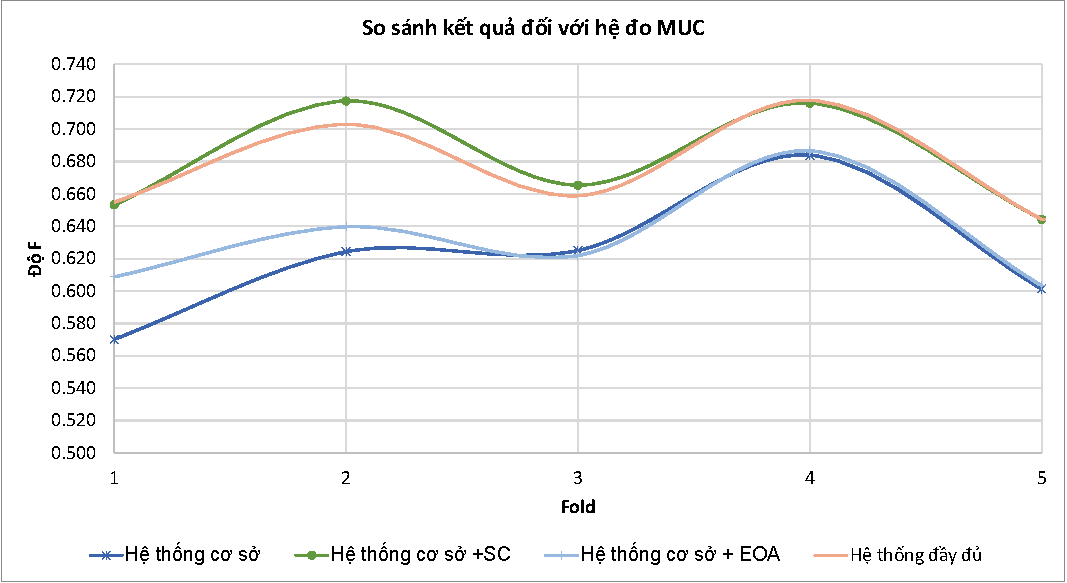
\includegraphics[scale=0.35]{charts/chart_muc.pdf}											
					\end{figure} 				
				\end{column}
				\begin{column}{0.4\textwidth}
				\end{column}
			\end{columns}
			\begin{columns}[t]
				\begin{column}{0.4\textwidth}
				\end{column}
				\begin{column}{0.6\textwidth}
					\begin{figure}[H] 
						\centering					
						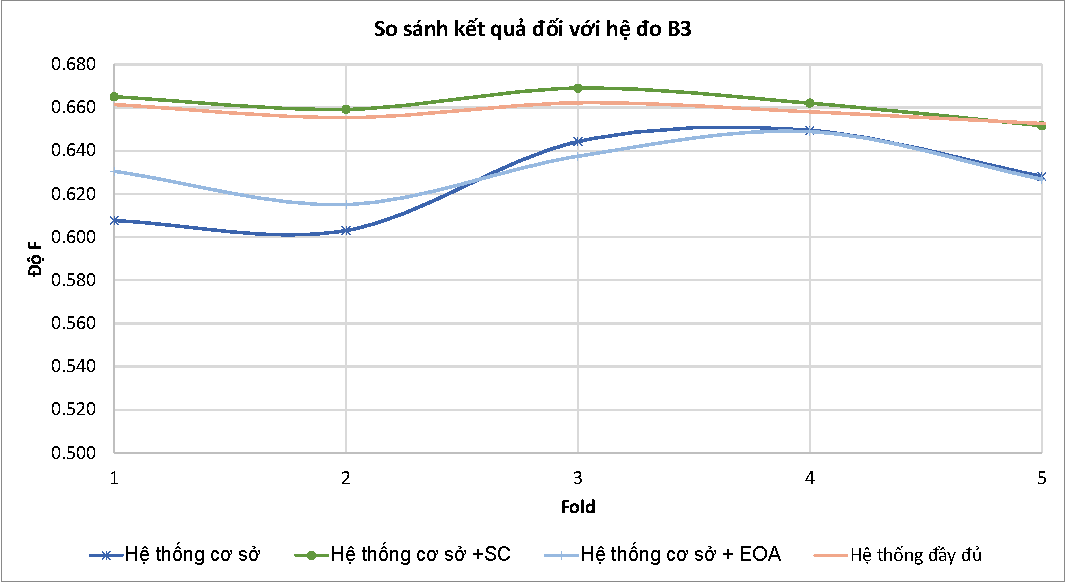
\includegraphics[scale=0.35]{charts/chart_b3.pdf}					
					\end{figure}
				\end{column}				
			\end{columns}						
		\end{frame}

		\begin{frame}[t]{Thực nghiệm và đánh giá (tt)}								
			\begin{columns}[t]
				\begin{column}{\textwidth}
					\begin{figure}[H] 			
						\centering					
						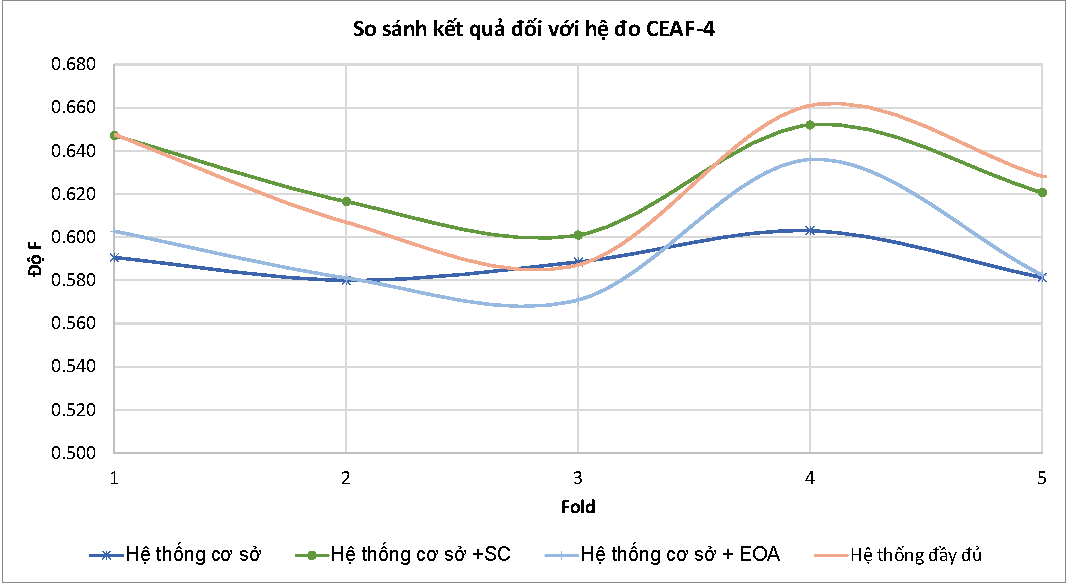
\includegraphics[scale=0.35]{charts/chart_ceaf4.pdf}										
					\end{figure} 				
				\end{column}
			\end{columns}
			\begin{columns}[t]
				\begin{column}{\textwidth}
					\begin{block}{Nhận xét}
						\footnotesize		
						\begin{itemize}
							\item{Đặc trưng liên quan đến Khai khoáng ý kiến đã ảnh hưởng tích cực đến kết quả}
							\item{Đặc trưng \textit{Tính nhất quán về ý kiến (SC)} đã có ảnh hưởng tương đối lớn đến hệ thống}
							\item{Đặc trưng \textit{Sự kết hợp giữa thực thể và từ chỉ ý kiến (EOA)} ít có ảnh hưởng tích cực đến hệ thống}
							\item{Việc kết hợp hai đặc trưng mới \textit{Tính nhất quán về ý kiến (SC)} và \textit{Sự kết hợp giữa thực thể và từ chỉ ý kiến (EOA)} vẫn còn gặp vấn đề}
						\end{itemize}			
					\end{block}
				\end{column}				
			\end{columns}						
		\end{frame}	

	\section{Tổng kết}
		\begin{frame}{Tổng kết}			
			\begin{block}{Kết quả đạt được}
				\begin{itemize}
					\item Từ những kiến thức về Phân giải đồng tham chiếu và Khai khoáng ý kiến, đưa ra được phương pháp giải quyết bài toán.
					\item Hiện thực hệ thống dựa trên phương pháp đề xuất, cho kết quả đầu ra khả quan.				
				\end{itemize}
			\end{block}
			\begin{block}{Khó khăn, hạn chế}
				\begin{itemize}
					\item Dữ liệu tự thu thập có nhiều câu phức tạp, gây ảnh hưởng đến các đặc trưng liên quan Khai khoáng ý kiến. 
					\item Do giới hạn về thời gian nên chưa kịp thử nghiệm cho tiếng Việt.				
				\end{itemize}
			\end{block}
		\end{frame}
	
		\begin{frame}{Tổng kết (tt)}			
			\begin{block}{Hướng phát triển}
				\begin{itemize}
					\item Tìm thêm các đặc trưng mới liên quan đến Khai khoáng ý kiến để tăng hiệu suất hệ thống.
					\item Cải thiện đặc trưng \textit{Sự kết hợp giữa thực thể và từ chỉ ý kiến}.
					\item Thử nghiệm cho tiếng Việt.
				\end{itemize}
			\end{block}
		\end{frame}

		\begin{frame}{Câu hỏi}
			\Huge
			\centering
			\fontsize{30pt}{30}\selectfont
			\textit{Câu hỏi}
		\end{frame}

\end{document}